\documentclass[12pt]{article}
\usepackage{url,graphicx,tabularx,array,geometry,enumitem,amsmath}
\setlength{\parskip}{1ex} %--skip lines between paragraphs
\setlength{\parindent}{0pt} %--don't indent paragraphs

%-- Commands for header
\renewcommand{\title}[1]{\textbf{#1}\\}
\renewcommand{\line}{\begin{tabularx}{\textwidth}{X>{\raggedleft}X}\hline\\\end{tabularx}\\[-0.5cm]}
\newcommand{\leftright}[2]{\begin{tabularx}{\textwidth}{X>{\raggedleft}X}#1%
& #2\\\end{tabularx}\\[-0.5cm]}
\def\ci{\perp\!\!\!\perp}


%\linespread{2} %-- Uncomment for Double Space
\begin{document}

\title{Digital Signal Processing - Assignment 9}
\line
\leftright{\today}{Stephanie Lund (2555914)\\Stalin Varanasi (2556235)} %-- left and right positions in the header

\section*{Exercise 1}

\subsection*{1.1}
See file $hw9.m$

\subsection*{1.2}
See file $pre.m$\\

This a filter which is used to emphasize the higher frequencies over the lower frequencies. The purpose of pre-emphasis is to counterbalance that low frequencies are much more prominent than high frequencies in speech.

\subsection*{1.3}
See file $windowing.m$\\

The purpose of windowing in general is to capture local properties of the signal at a particular time.\\
The window size is chosen as a compromise between time and frequency resolution. In this case, 25ms is chosen because it allows very good time resolution, and is just long enough to allow sufficient frequency resolution to identify speech sounds.

\subsection*{1.4}
See file $hw9.m$\\

The resulting plot is as follows:\\
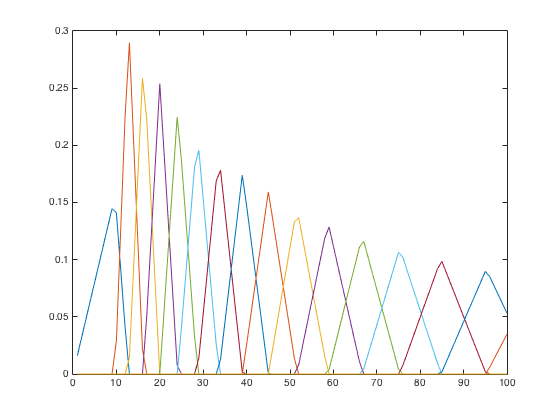
\includegraphics[scale=0.8]{hw9-1.png}

\subsection*{1.5}
See file $hw9.m$

The spectrogram is as follows:\\

\includegraphics[scale=0.8]{hw9-2.png}

The Y-axis represents time and the x-axis ,frequency.The amplitude is represented by the color of the pixel.We can see hikes of frequencies at regular intervals of time.

\subsection*{1.6}
See file $hw9.m$.

The resulting image is:\\
\includegraphics[scale=0.8]{hw9-3.png}

The image has frequency hikes at specific intervals of time because, the sound is from a keyboard played one key at each regular interval.


\end{document}
